

\chapter{Results}
% o Present all results here
% o No discussion, no interpretation, no evaluation etc.
% o Figures / Tables
%  Use wisely
%  Consult your supervisor about what to present
%  put very large and detailed tables rather in the appendix
%  put source code in appendix
% o Do not write down all data from table in text, but put them in relation to each other
% o Help reader to understand tables & graphs and highlight important and/or interesting data
% o Present an assessment of uncertainties

On the second day of working with the filled rods the one containing liquid \textbf{\#6} broke (leakage).
It happened when delicately knocking it against on the table while standing upright.
This was intended to mobilise bubbles that sticked to the wall and make them travel vertically to on end of the rod. (see tabular \ref{tab:bubbles})
The plastic stopper on the lower end came loose.
The rod containing filling \textbf{\#6} was not replaced.
Consequently, all CT and MRI images show only 16 rods.

\section{Obtained MRI and CT scans}
Figure \ref{fig:coronal} shows a coronal view of the 16 rods filled with the tested liquids.
(in figure \ref{fig:axial_MR} a plastic bottle filled with water has been placed there instead (see figure \ref{fig:axial_CT_pane}).)
 
\begin{figure}[!tbp]
  \begin{subfigure}[b]{\textwidth}
    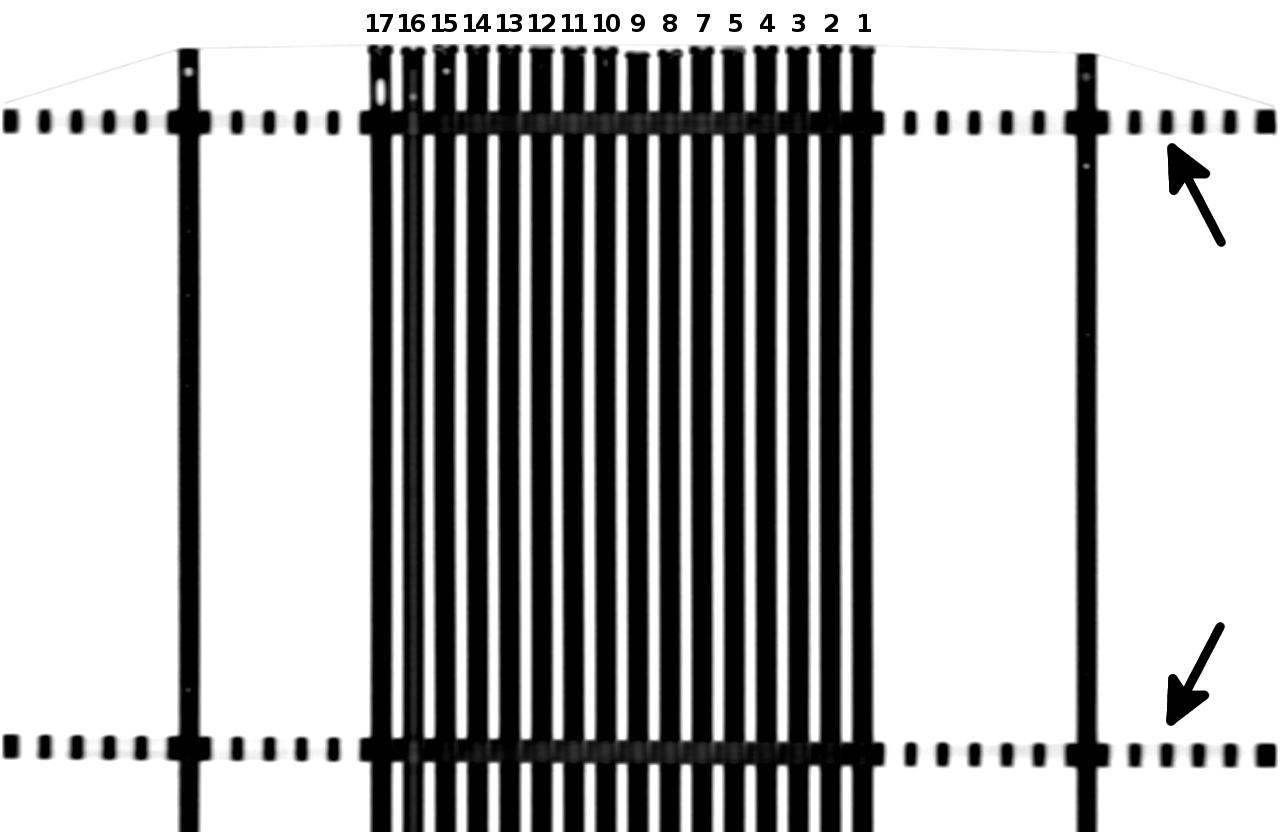
\includegraphics[width=\textwidth]{slicer3D/full_phantom/coronal_CT_cropped-arrow.png}
    \caption{CT: periodic black lines in upper and lower part of image (arrows) show plastic panes from above); rods have been fixed with adhesive tape (faint line across upper end of rods); differences in signal intensity (brightness) hardly noticeable, but air bubbles visible at upper end}
    \label{fig:coronal_CT}
  \end{subfigure}
  \begin{subfigure}[b]{1\textwidth}
    
\includegraphics[width=1\textwidth]{slicer3D/full_phantom/coronal_MR_cropped.png}
    \caption{MR: rods appear to be thinner, because only the liquid filling is visible; plastic (rods and panes) are not visible}
    \label{fig:coronal_MR}
  \end{subfigure}
  \caption{Coronal CT/MRI (inverted colours; same scale; cropped images): images of 16 rods (tested liquids, numbering starting from the right, \#6 excluded) + 2 reference rods (filled with water) on the sides; liquids result in different signal intensity (brightness)}
  \label{fig:coronal}
\end{figure}

\begin{figure}[!tbp]
  \begin{subfigure}[b]{\textwidth}
    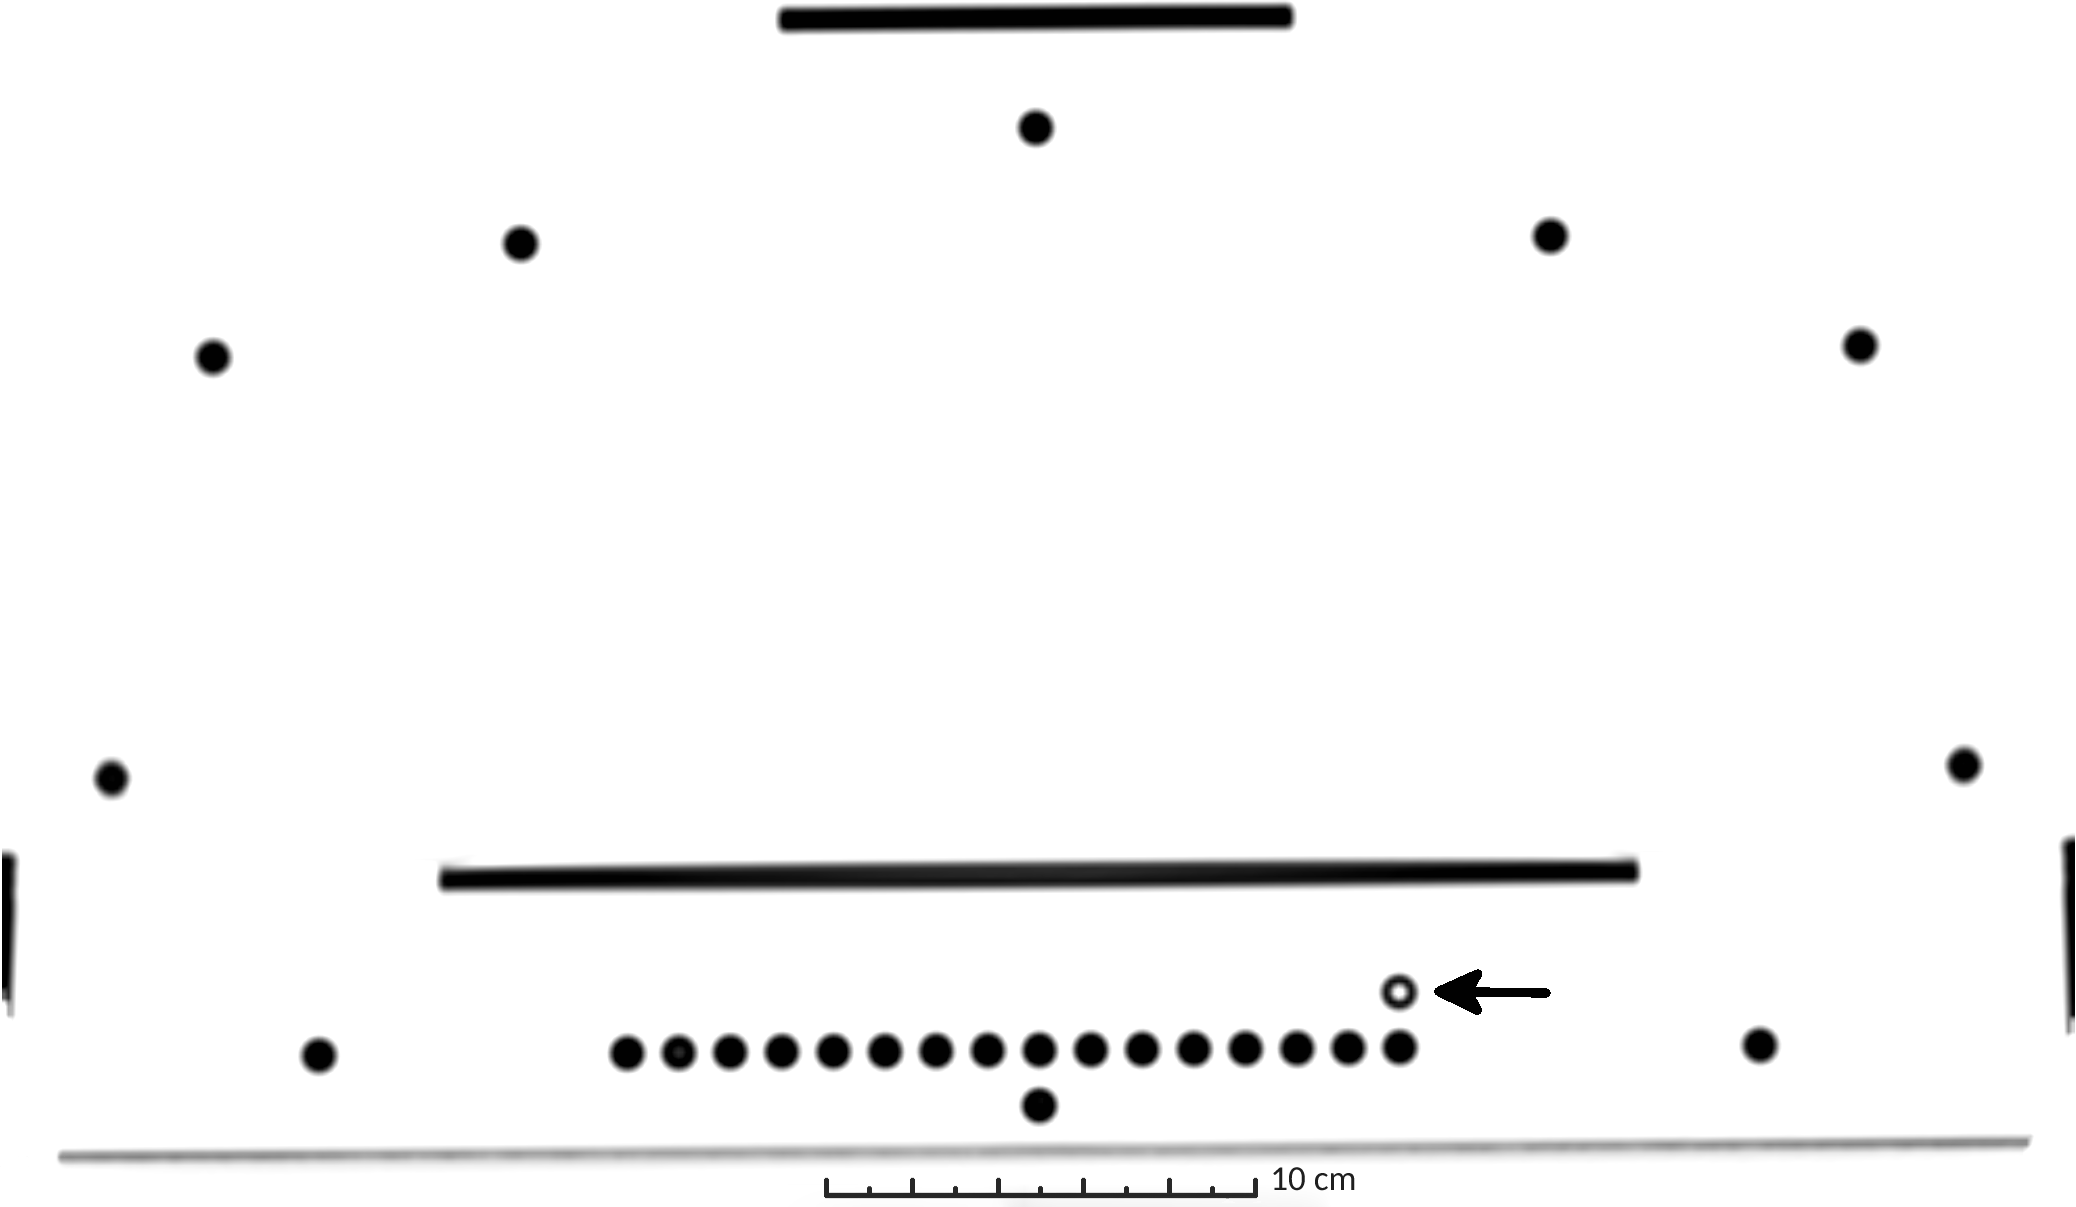
\includegraphics[width=\textwidth]{slicer3D/full_phantom/axial_CT_rods-arrow.png}
    \caption{CT: black bars just above tested rods, at the very top and to the sides show plastic parts of the phantom holding it together; faint grey line below tested rods shows table on which phantom was positioned during imaging}
    \label{fig:axial_CT_rods}
  \end{subfigure}
  \begin{subfigure}[b]{\textwidth}
    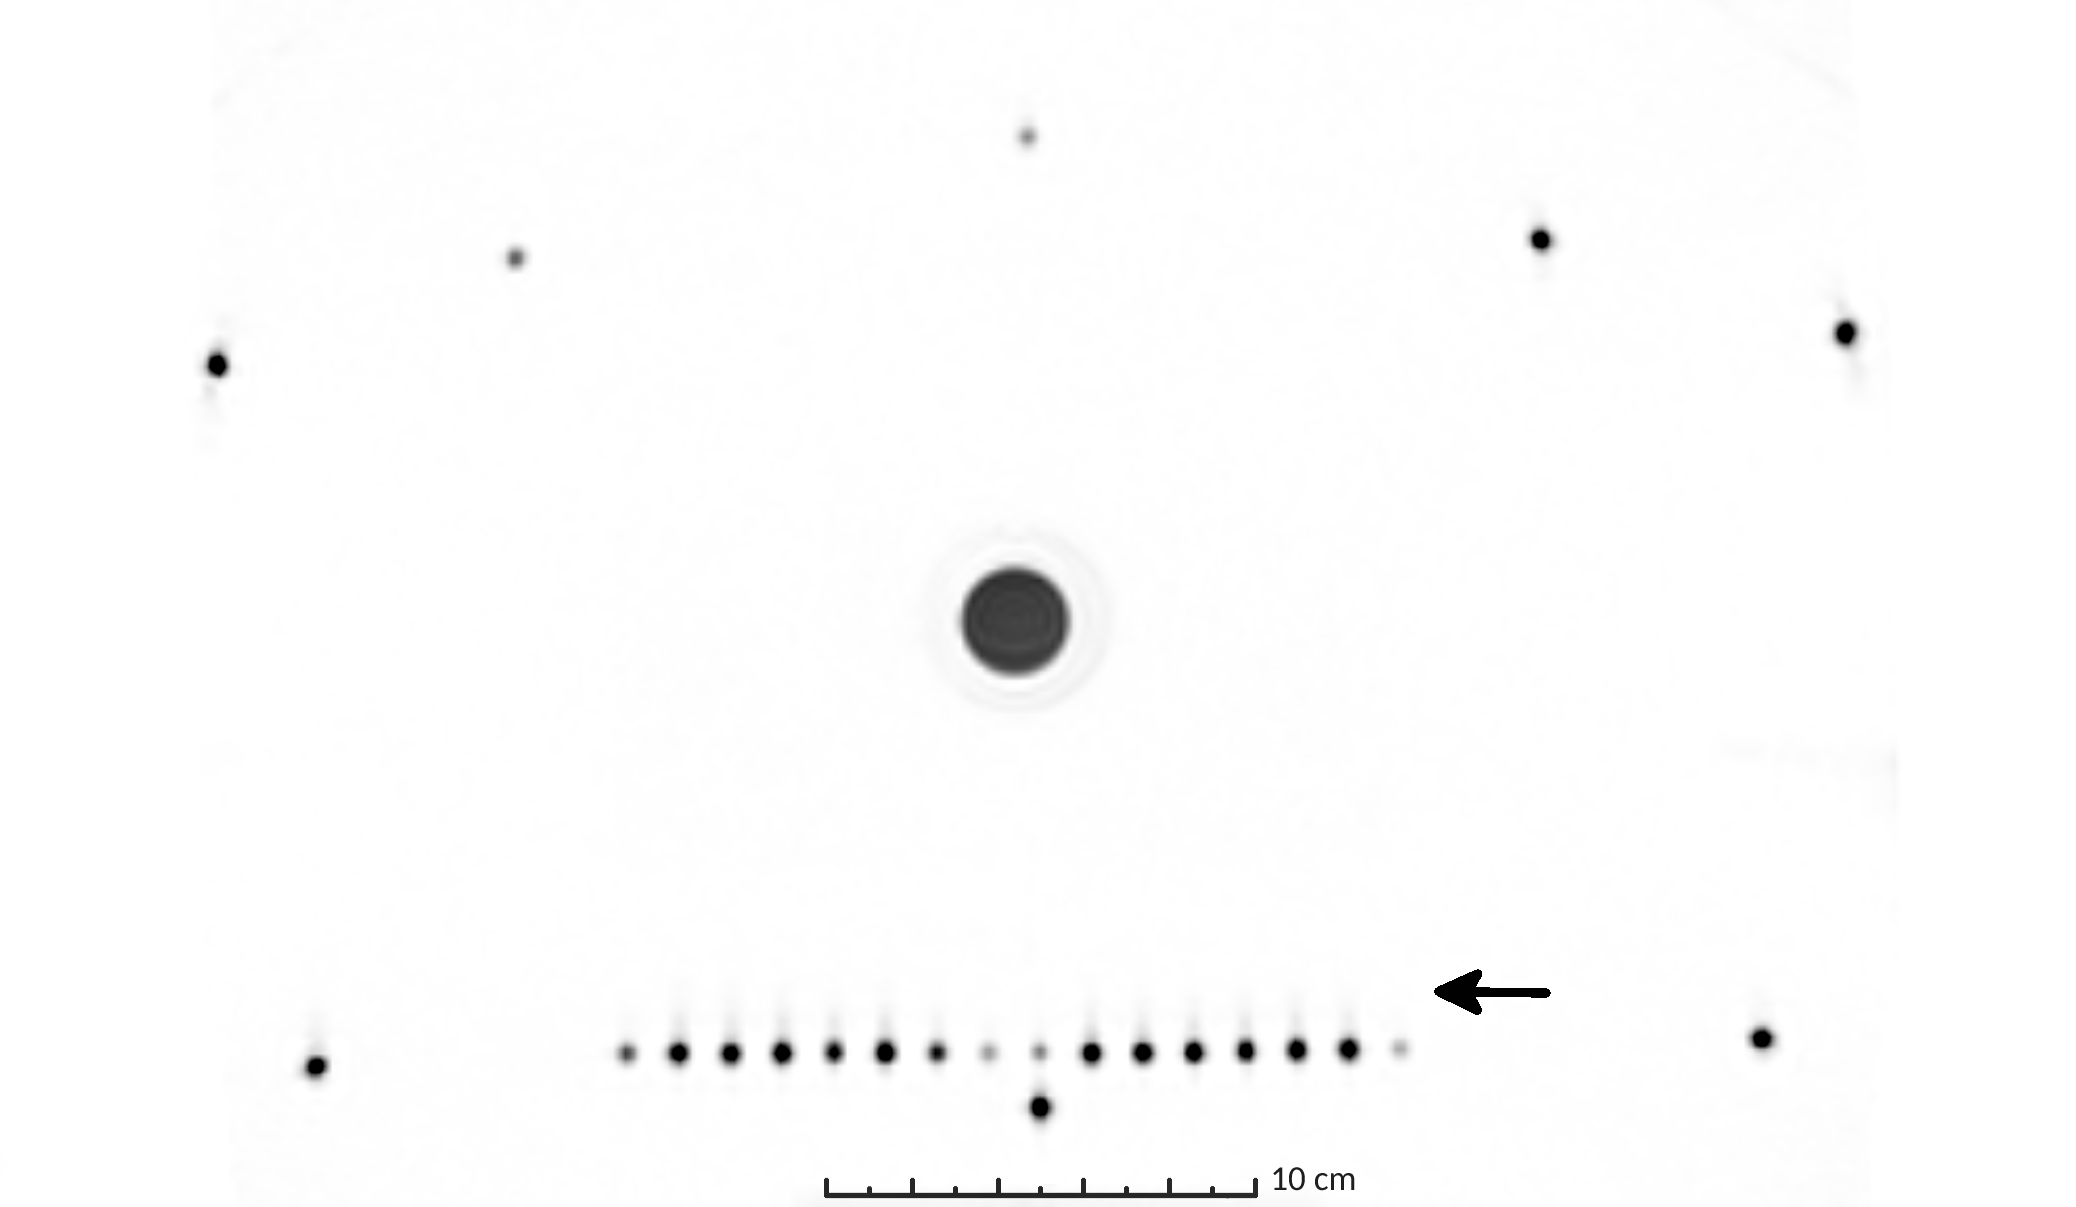
\includegraphics[width=\textwidth]{slicer3D/full_phantom/axial_MR-arrow.png}
    \caption{MRI: black circle in middle shows water bottle which was placed in the middle of the phantom (necessary for MRI scanner to start imaging)}
    \label{fig:axial_MR}
  \end{subfigure}
  \caption{axial CT/MRI (inverted colours, same scale): images of 16 rods (tested liquids, numbering starting from the right, \#6 excluded); surrounded by reference rods (filled with water) and one empty rod (marked with arrow) which is not visible on MRI scans}
  \label{fig:axial}
\end{figure}


\section{Tested solutions}

\subsection{Visibility on CT/MRI scans}

CT images show little differences between the tested liquids. The plastic rods themselves result in brighter pixels than any of the tested solutions.

On MRI scans most liquids had a mean and a max brightness value above $1000$ (see table \ref{tab:visibility}).\\
Only \textbf{\#1}, \textbf{\#9}, \textbf{\#10}, \& \textbf{\#17} resulted in significantly less signal.


\begin{table}[]
\centering
\begin{tabular}{@{}lllllll@{}}
\toprule
No. & Min  & Max  & Mean   & Median & RMS    & $\sigma$   \\ \midrule
1   & 182  & 371  & 288    & 269    & 296,3  & 69,8   \\
2   & 1044 & 1921 & 1443,8 & 1405   & 1477,3 & 312,9  \\
3   & 941  & 2075 & 1451,2 & 1394,5 & 1508,9 & 413,2  \\
4   & 1176 & 1709 & 1440   & 1437,5 & 1458,6 & 232,5  \\
5   & 1125 & 2111 & 1583,8 & 1549,5 & 1623   & 355    \\
7   & 971  & 2241 & 1466,8 & 1316   & 1540,6 & 471,2  \\
8   & 1459 & 1947 & 1704   & 1705   & 1713,5 & 180,5  \\
9   & 385  & 584  & 486,8  & 489    & 495,6  & 93     \\
10  & 247  & 502  & 343,6  & 266    & 361,1  & 111    \\
11  & 830  & 1268 & 1036,2 & 1023,5 & 1049   & 163,2  \\
12  & 1158 & 2211 & 1648,8 & 1613   & 1695,2 & 394,2  \\
13  & 836  & 1657 & 1146,8 & 1047   & 1190,9 & 321,2  \\
14  & 800  & 2062 & 1383   & 1335   & 1461,7 & 473,1  \\
15  & 1156 & 1829 & 1476,2 & 1460   & 1501,2 & 272,7  \\
16  & 1102 & 1967 & 1509   & 1483,5 & 1543,8 & 325,8  \\
17  & 356  & 938  & 629,6  & 602    & 668,1  & 223,6  \\ \bottomrule
\end{tabular}
\caption{liquid visibility on MRI scan}
\label{tab:visibility}
\end{table}

% 
% \begin{table}[]
% \centering
% \begin{tabular}{@{}l|rrr@{}}
% No.	& brightest MRI pixel	& darkest CT pixel [$HU$]	& CT @ brightest pixel MRI	\\
% \toprule
% \#1	& 342			& -6		& 7		\\
% \#2	& 1777			& 31		& 31		\\
% \#3	& 1771		& 5		& 8			\\
% \#4	& 1589		& 62		& 62			\\
% \#5	& 1691		& -6		& -2			\\
% \#6	&  \multicolumn{3}{c}{\textit{------------------------ rod was leaking ---------------------------}}	\\
% \#7	& 1725		& 7		& 20			\\
% \#8	& 1868		& -40		& 43			\\
% \#9	& 514		& -11		& -11			\\
% \#10	& 477		& 1		& 1			\\
% \#11	& 1246		& -12		& 7			\\
% \#12	& 1794		& 18		& 18			\\
% \#13	& 1416		& 152		& 157			\\
% \#14	& 1814		& 4		& 4			\\
% \#15	& 1705		& 11		& 32			\\
% \midrule
% \#16	& 1848		& -196		& -196			\\
% \#17	& 836 		& 123		& 129			\\
% \bottomrule
% \end{tabular}
% \caption{liquid visibility}
% \label{tab:visibility}
% \end{table}

\subsection{Mechanical properties of solutions}
A suitable filling would yield good image contrast in CT and MRI and acceptable mechanical properties.

The liquids were filled in a rod each and observed for several months. Some solutions produced air bubbles, which would eventually lead to incorrect calculations.
Each rod was free of bubbles after sealing. The amount of gas inside the rods was measured after 2 months. Ideally, tilting the entire phantom slightly should be enough to fix all rods in the phantom at the same time.
In some of the tested rods the produced air bubbles would stick to the wall. Only after gently hitting the rod they would start moving (see table \ref{tab:bubbles}).

\begin{table}[]
\centering
\begin{tabular}{l|lc|lc|lc}
    & \multicolumn{2}{c}{\textit{after 1 day}} 	& \multicolumn{2}{c}{\textit{after 2 days}}	& \multicolumn{2}{c}{\textit{after 1 week}}	\\ 
No. & bubbles	& hit req.	& bubbles 	& hit req.	& bubbles 	& hit req.	\\
\toprule
\#1   & yes	& no		& no		&		& no		&		\\
\#2   & yes	& yes		& no		&		& no		&		\\
\#3   & yes	& yes		& no		&		& no		&		\\
\#4   & yes	& yes		& no		&		& no		&		\\
\#5   & yes	& no		& yes		& no		& no		&		\\
\#6   & yes	& no		& \multicolumn{4}{l}{-----------------\textit{ rod was leaking }------------------}	\\
\#7   & yes	& no		& yes		& no		& yes		& no		\\
\#8   & no	&		& no		&		& no		&		\\
\#9   & no	&		& no		&		& no		&		\\
\#10  & no$^1$	&		& yes		& yes		& yes		& yes		\\
\#11  & no	&		& yes,		& \textit{sticked to wall} &	 yes	& yes\\
\#12  & yes	& yes		& yes,		& \textit{sticked to wall} &	 yes	& yes\\
\#13  & yes	& yes		& yes,		& \textit{sticked to wall} &	 yes	& yes\\
\#14  & no	&   		& yes		& no		& yes		& yes		\\
\#15  & no	&   		& no		&		& no		&		\\
\#16  & no	&   		& no		&		& no		&		\\
\#17  & no	&   		& no		&		& no		&		\\
\bottomrule
\end{tabular}
\begin{tabular}{l|lr}
\multicolumn{3}{c}{}								\\
& \multicolumn{2}{c}{\textit{after 2 months}}					\\ 
No. & length of trapped bubble $l$ [$mm$] 	& approx. volume $V$ [$mm^3$]	\\
\toprule
\#1   & 2					& 25.13				\\
\#2   & 1.8					& 22.62				\\
\#3   & 1+1 (air blockage, at lower end)	& 25.13				\\
\#4   & 4					& 50.27				\\
\#5   & 1.5 (many small bubbles)		& 18.85				\\
\#6   & \multicolumn{2}{c}{-----------------------------\textit{ rod was leaking }------------------------------}\\
\#7   & 2 (many small bubbles)			& 25.13				\\
\#8   & 2.3					& 28.90				\\
\#9   & 3					& 37.70				\\
\#10  & 2.4					& 30.16				\\
\#11  & 2					& 25.13				\\
\#12  & 2					& 25.13				\\
\#13  & 2.3					& 28.90				\\
\#14  & 1.5+0.5 (big immobile bubble, at center)	& 25.13				\\
\#15  & 3.4 (agar gel dried)			& 42.73				\\
\#16  & 0					& 0.00				\\
\#17  & 0.5					& 6.28				\\
\bottomrule
\end{tabular}
\caption{solutions, observations}
\label{tab:bubbles}
\end{table}

Knowing the inner diameter $d$ of the rods we can easily approximate the volume of gas trapped:

\begin{align}
 V = \frac{d^2}{4}\cdot \pi \cdot l
\end{align}

% \begin{table}[p]
%   \centering
%   \rotatebox{90}{
%     \begin{minipage}{\textheight}\footnotesize
%       \centering
%       \begin{tabular}{@{}r|cccc|ccccrrr@{}}
% 	    & \multicolumn{4}{c}{\textit{after 1 day}}	& \multicolumn{4}{c}{\textit{after 2 days}}			& \multicolumn{4}{c}{\textit{after 1 week}}&		 \multicolumn{4}{c}{\textit{after 2 months}}                 \\ 
% 	    & \multicolumn{4}{c}{} 			& \multicolumn{4}{c}{}                             \\
% 	Nr. & bubbles	& angle		& hit req.	& bubbles 	& angle		& hit req.	&  \\
% 	\toprule
% 	1   & yes	& $10^o$	& no		& no		&		&		&   \\
% 	2   & yes	& $40^o$	& yes		& no		&		&		&   \\
% 	3   & yes	& $40^o$	& yes		& no		&		&		&   \\
% 	4   & yes	& $80^o$	& yes		& no		&		&		&   \\
% 	5   & yes	& $10^o$	& no		& yes		& $10^o$	& no		&   \\
% 	6   & yes	& $10^o$	& no		& \multicolumn{5}{r}{--------------\textit{ rod was leaking }------------} \\
% 	7   & yes	& $10^o$	& no		& yes		& $10^o$	& no		&   \\
% 	8   & no	&		&   		& no		&		&		&   \\
% 	9   & no	&		&   		& no		&		&		&   \\
% 	10  & no$^1$	&		&   		& yes		& $20^o$	& yes		&   \\
% 	11  & no	&		& yes		& yes		& \multicolumn{4}{r}{---\textit{ bubbles sticked to wall }---} \\
% 	12  & yes	& $60^o$	& yes		& yes		& \multicolumn{4}{r}{---\textit{ bubbles sticked to wall }---} \\
% 	13  & yes	& $80^o$	& yes		& yes		& \multicolumn{4}{r}{---\textit{ bubbles sticked to wall }---} \\
% 	14  & no	&		&   		& yes		& $40^o$	& no		&   \\
% 	15  & no	&		&   		& no		&		&		&   \\
% 	16  & no	&		&   		& no		&		&		&   \\
% 	17  & no	&		&   		& no		&		&		&   \\
% 	\bottomrule
%       \end{tabular}
%       \caption{Messwerte}
%       \label{tab:wirkungsgrad}
%     \end{minipage}
%   }
% \end{table}

\section{Distortion assessment}
All results were obtained by manually cropping the 3D image to depict only a single rod.

\todo{add slice which shows particular problem (e.g. high distortion, air bubble or artefact resulting in extra-hihg distortion value)}
\todo{rename xy axis, x-axis = distance from middle instead of slice number}
\todo{discuss what is visible on the graphs in discussion section}
\subsection{Distortion}

\vspace{4cm}
\textit{table showing distortion along z axis (isocentre to image border)}
\vspace{2cm}

\begin{figure}[!tbp]
  \begin{subfigure}[b]{0.32\textwidth}
    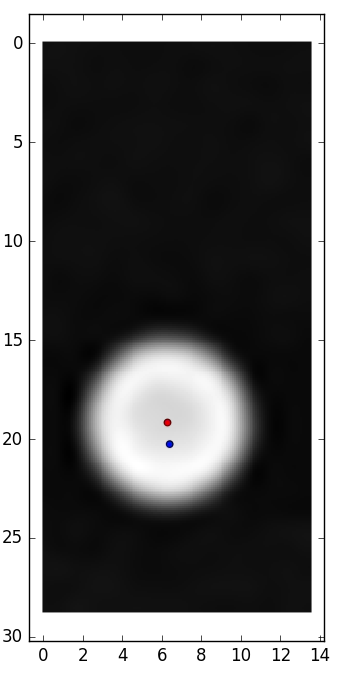
\includegraphics[scale=0.55]{python/centroid/CT_x100@0_centroids.png}
    \caption{CT @ 0}
    \label{fig:CT_x100_centroids@0}
  \end{subfigure}
  \begin{subfigure}[b]{0.32\textwidth}
    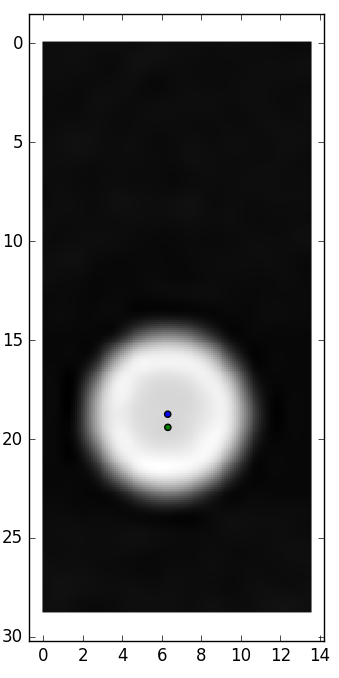
\includegraphics[scale=0.55]{python/centroid/CT_x100@150_centroids.png}
    \caption{CT @ 150}
    \label{fig:CT_x100_centroids@150}
  \end{subfigure}
  \begin{subfigure}[b]{0.32\textwidth}
    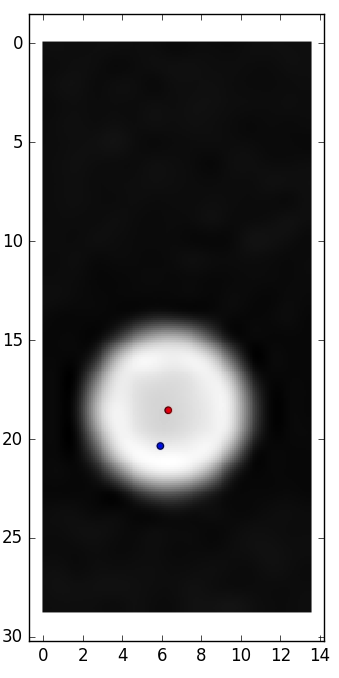
\includegraphics[scale=0.55]{python/centroid/CT_x100@304_centroids.png}
    \caption{CT @ 304}
    \label{fig:CT_x100_centroids@304}
  \end{subfigure}
  \begin{subfigure}[b]{0.32\textwidth}
    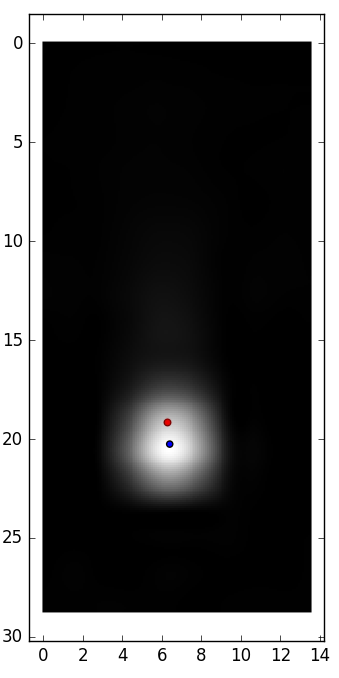
\includegraphics[scale=0.55]{python/centroid/MR_x100@0_centroids.png}
    \caption{MRI @ 0}
    \label{fig:MR_x100_centroids@0}
  \end{subfigure}
  \begin{subfigure}[b]{0.32\textwidth}
    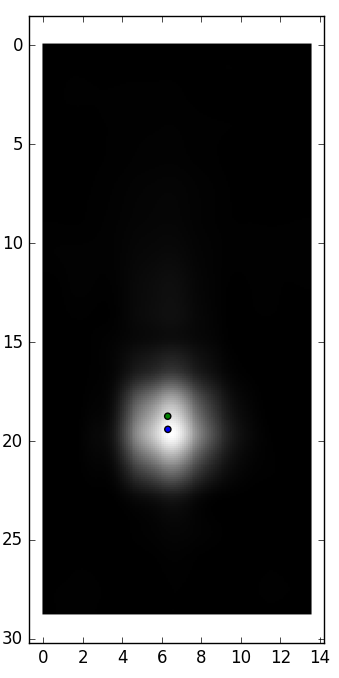
\includegraphics[scale=0.55]{python/centroid/MR_x100@150_centroids.png}
    \caption{MRI @ 150}
    \label{fig:MR_x100_centroids@150}
  \end{subfigure}
  \begin{subfigure}[b]{0.32\textwidth}
    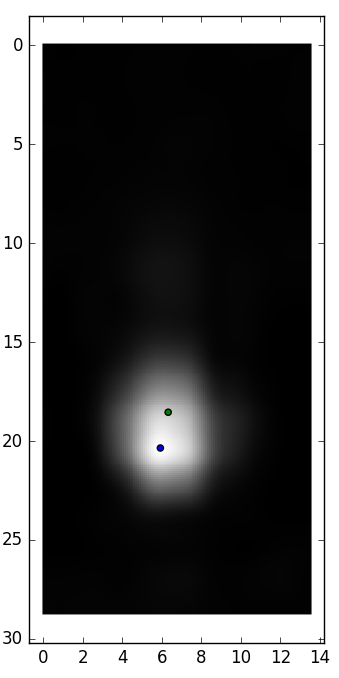
\includegraphics[scale=0.55]{python/centroid/MR_x100@304_centroids.png}
    \caption{MRI @ 304}
    \label{fig:MR_x100_centroids@304}
  \end{subfigure}
  \caption{MRI x100; blue dot centroid MRI, green dot centroid CT (same scale);\\ slice 150 is approximately at the isocentre, 0 on the very end of the image, 304 close to an air bubble}
  \label{fig:MR_x100_centroids}
\end{figure}

\clearpage

\subsection{DC}

\begin{figure}[!bp]
  \centering
  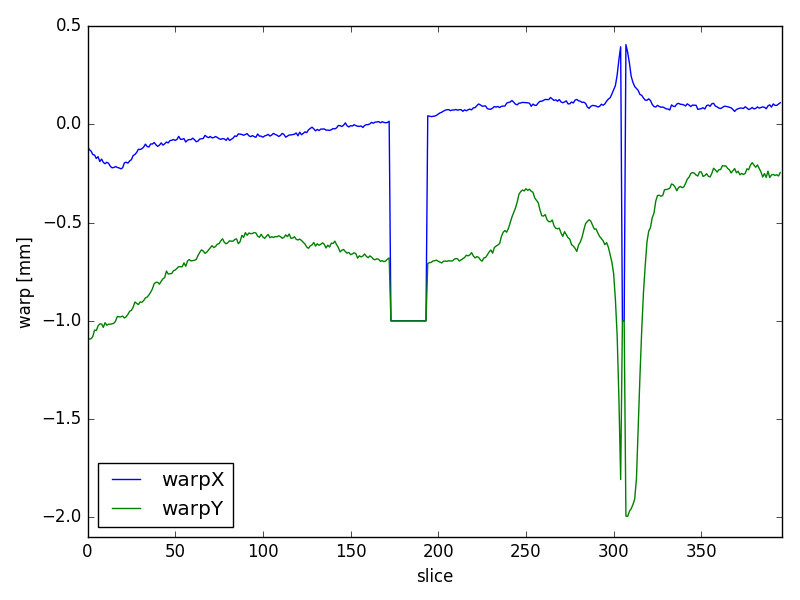
\includegraphics[scale=0.6]{python/warp/warpXY_x100--.png}
  \caption{warp XY [$mm$], CT-MRI x100}
  \label{fig:warpXY_x100}
\end{figure}

\begin{figure}[!tp]
    \centering
    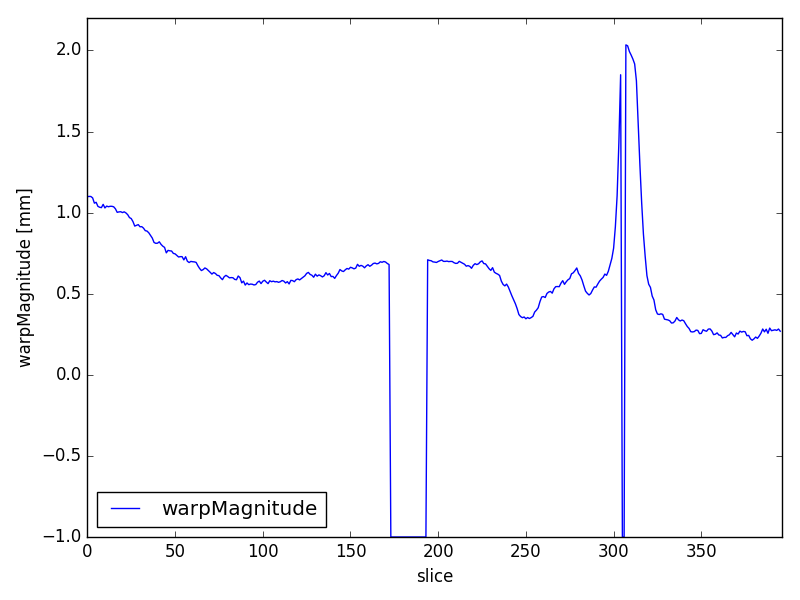
\includegraphics[scale=0.6]{python/warp/warpMagnitude_x100--.png}
    \caption{warp Magnitude [$mm$], CT-MRI x100}
    \label{fig:warpMagnitude_x100}
\end{figure}
\begin{figure}[!bp]
    \centering
    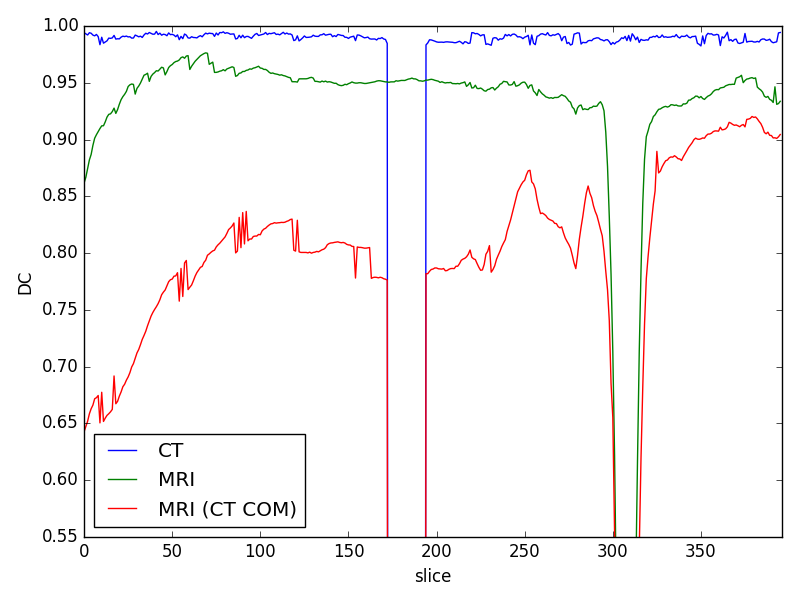
\includegraphics[scale=0.6]{python/dice/CT_MR_x100_DC.png}
    \caption{DC (optimised) for CT \& MRI \& MRI (using CT COM)}
    \label{fig:CT_MR_x100_DC}
\end{figure}

\begin{figure}[!tp]
    \centering
    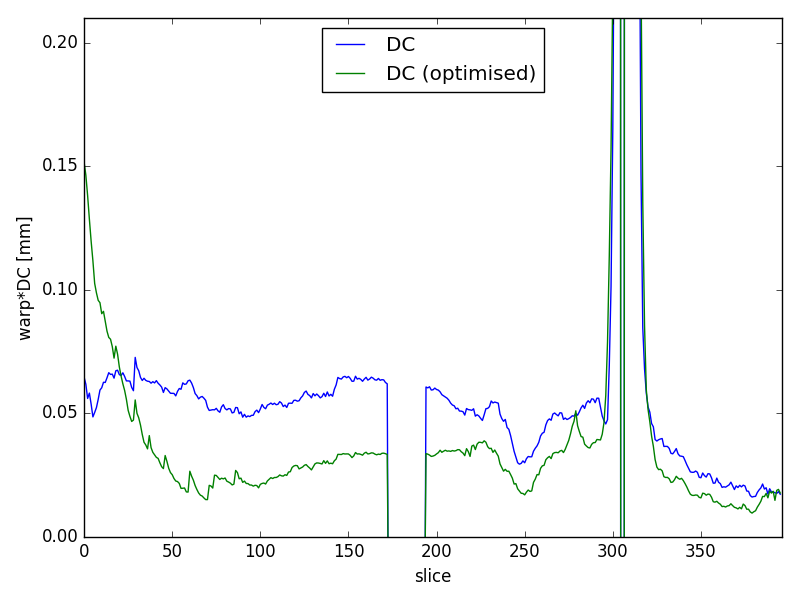
\includegraphics[scale=0.6]{python/warpDC/warpDC_x100.png}
    \caption{artificial indicator warp*DC using real DC and optimised DC of MRI x100}
    \label{fig:warpDC_x100}
\end{figure}
\begin{figure}[!bp]
  \centering
  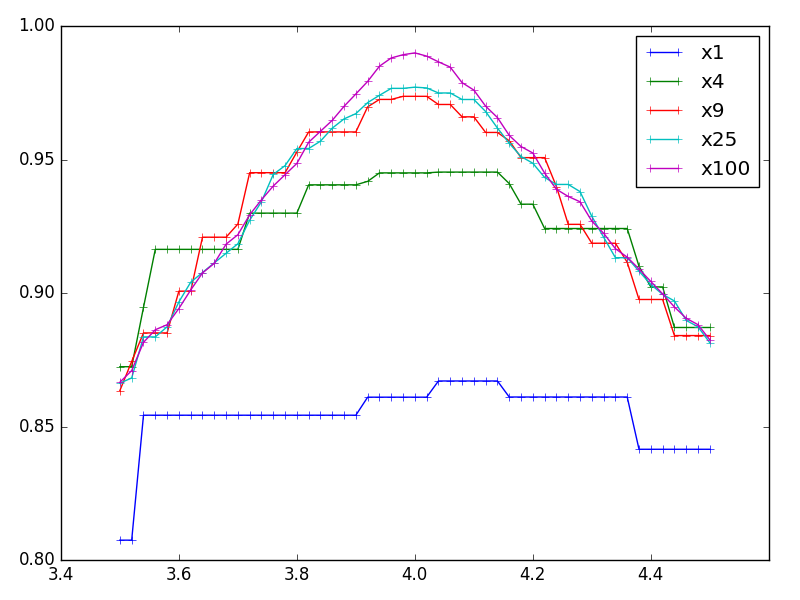
\includegraphics[scale=0.6]{python/dice/CT-51iter.png}
  \caption{CT: DC of varied radii \& resolutions}
  \label{fig:CT_dc}
\end{figure}

\begin{figure}[!tbp]
  \begin{subfigure}[b]{\textwidth}
    \centering
    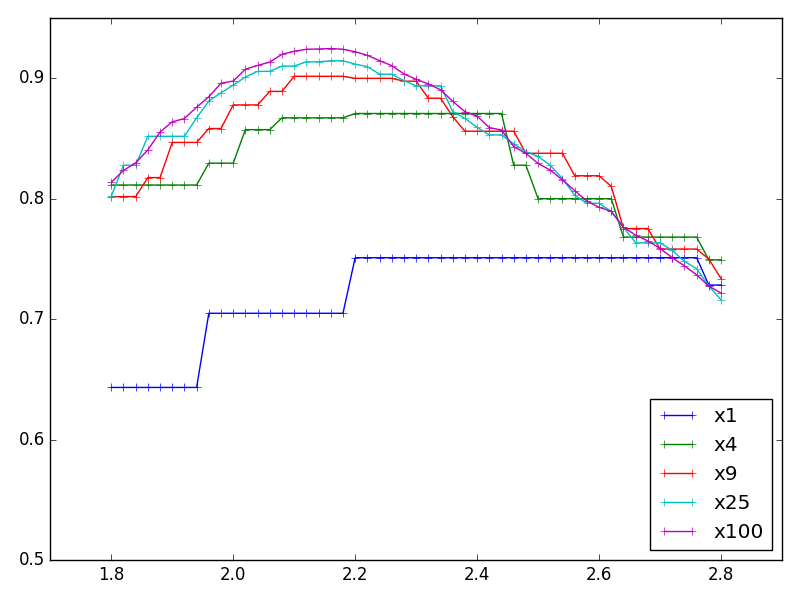
\includegraphics[scale=0.6]{python/dice/MR-51iter.png}
    \caption{MRI: DC of varied radii \& resolutions}
    \label{fig:MR_dc-opti}
  \end{subfigure}
  \begin{subfigure}[!b]{\textwidth}
    \centering
    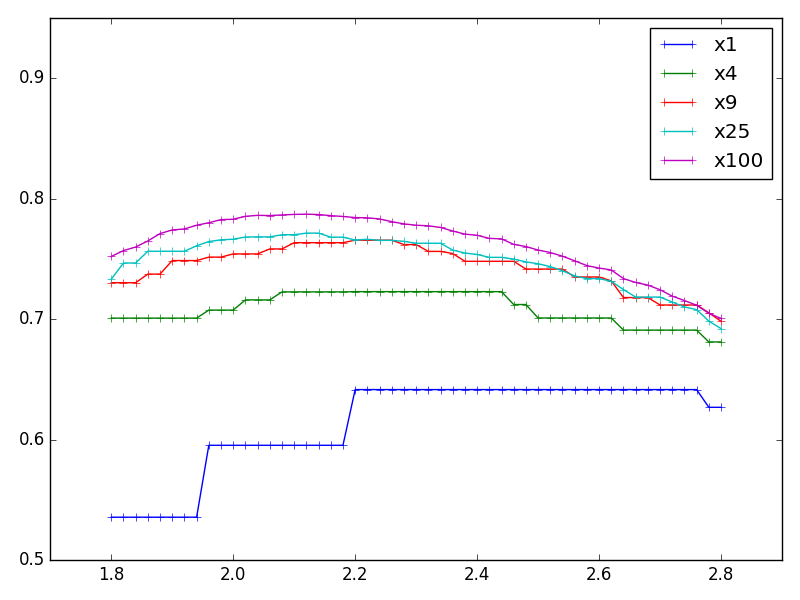
\includegraphics[scale=0.6]{python/dice/MR_CT-COM_51iter.png}
    \caption{MRI: DC of varied radii \& resolutions (using CT-COM)}
    \label{fig:MR_CT-COM_dc-opti}
  \end{subfigure}
  \caption{}
  \label{fig:MR_dc}
\end{figure}


The obtained dice coefficient varies not only because of the circle's centre and the radius, it also depends on the images resolution.
Figure \ref{fig:CT_dc} and \ref{fig:MR_dc} show the DC (optimised) obtained using CT and MRI scans over resample rate.

\todo{include table with actual RESULTS that are spit out by script and reference to python code (which will be in appendix)}
\todo{PIOTR: create colour coded images}

% \begin{figure}[!tbp]
%   \begin{subfigure}[b]{\textwidth}
%     \centering
%     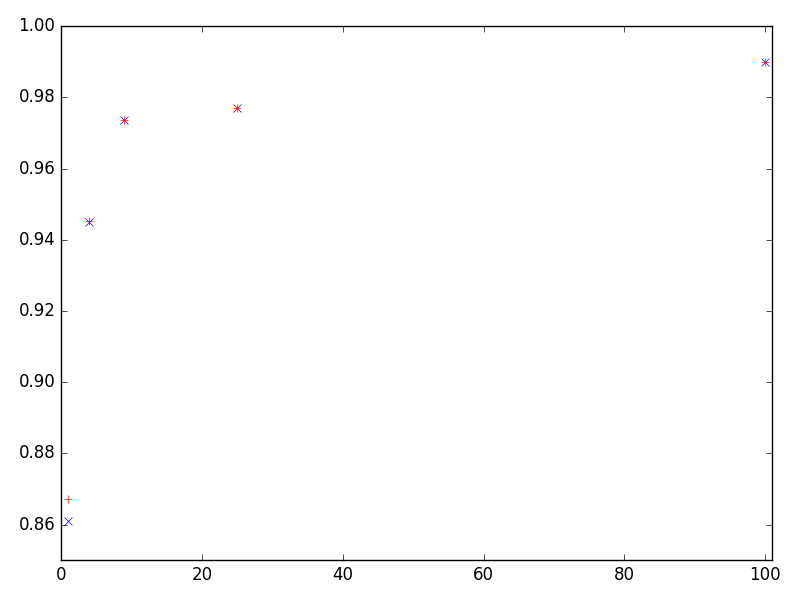
\includegraphics[scale=0.65]{python/dice/CT_dice-comparison_fast-51iter.png}
%     \caption{CT: x1, x4, x9, x16, x25, x100}
%     \label{fig:MR_dice-comp}
%   \end{subfigure}
%   \begin{subfigure}[b]{\textwidth}
%     \centering
%     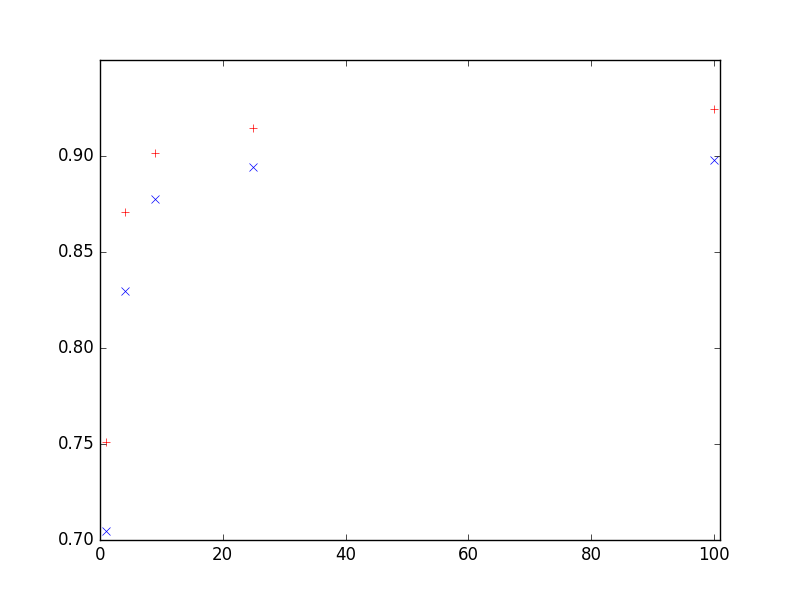
\includegraphics[scale=0.65]{python/dice/MR_dice-comparison_fast-51iter.png}
%     \caption{MRI: x1, x4, x9, x16, x25, x100}
%     \label{fig:MR_dice_comp}
%   \end{subfigure}
%   \caption{}
%   \label{fig:dice_com}
% \end{figure}

% image of COM shift